\documentclass{beamer}
\usetheme{metropolis}           % Use metropolis theme
\usepackage{blindtext}
\usepackage{enumitem}
\usepackage{chemformula}




\title{Phosphorus Release from Eroded Soil in the Aquatic Systems}
\date{\today}
\author{Antti-Jussi Kallio}
\institute{University of Helsinki}
\begin{document}
  \maketitle
  \section{Phosphorus cycle}
  \begin{frame}{Erosion}
    \begin{itemize}
    \item[*] Erosion control measures are applied all over the 			world,
    in many cases to protect the soil itself, or to reduce off-			site impacts  
    \item[*] Does controlling soil erosion inhibit aquatic 				eutrophication (rehev{\"o}ityminen)?
      \begin{itemize}
        \item[-] The main interest of our study
        \item[-] We study the mineralization pathways of \ch{Fe}, 			which is coupled to \ch{C}, \ch{S} and \ch{P} cycling.
        \item[-] The amount of \ch{C}, \ch{S}, aerobic vs 					anaerobic.
      \end{itemize}
    \end{itemize}
  \end{frame}
  \begin{frame}{Possible effects of eroded soil on eutrophication}
    \begin{itemize}
      \item[*] \small{(The following summarize applies to estuary 				  (murtovesi), or any \ch{SO4} rich recipient.)}
      \item[*] If the estuary receives a high input of \ch{Fe} 			  oxides and a modest level of dissolved \ch{P}, we may see 		  moderate levels of eutrophication.
      \item[*] The settling flux has a low \ch{C}/\ch{Fe} ratio 		  and the sediment is mainly in \ch{Fe} reduction state.
      \begin{itemize}
        \item[-] As a result the estuary may respond to erosion control because the \ch{P} concentrations are not maintained by strong \ch{P} release from the sediment due to coupled cycling of \ch{P} and \ch{Fe}. 
	  \end{itemize}
	  \item[*] The biotic fauna releases \ch{Fe} and \ch{P} from the oxides which then react with \ch{O2} in the aerobic estuary.
	  \begin{itemize}
		\item[-] No \ch{P} release from sediment to the aquatic system, keeps the "ferrous wheel" spinning.	
	  \end{itemize}	        
    \end{itemize}
  \end{frame}
  
  
  \begin{frame}{Possible effects of eroded soil on eutrophication}
    \begin{figure}
      \centering
      \caption{\footnotesize{\ch{Fe} and \ch{P} cycle in aerobic estuary}}
      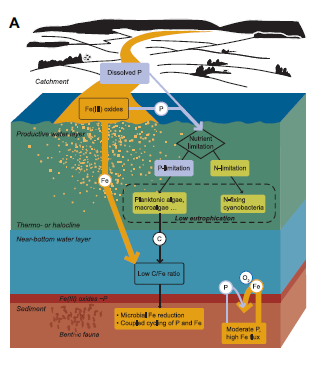
\includegraphics[scale=0.55]{../Kuvat/eutrophication_A.png}     
    \end{figure}
  \end{frame}
  
  \begin{frame}{Possible effects of eroded soil on eutrophication}
  \begin{itemize}
    \item[*] If erosion control takes place, typically dissolved \ch{P} increases as we reduce the input of \ch{Fe} oxides.
    \item[*] Increased bioavailable \ch{P} triggers algal (lev{\"a}) production, which increases the flux of organic \ch{C} to the sediment surface $\rightarrow$ \ch{SO4} reduction becomes important
    \item[*] The lowered flux of \ch{Fe} oxides means higher \ch{C}/\ch{Fe} ratio.
    \item[*] When \ch{SO4} reduction rates increase, more of the sediment \ch{Fe} is transformed to non-sorptive \ch{Fe} sulfides $\rightarrow$ massive release of \ch{Fe}-bound \ch{P} stored in sediments.        
  \end{itemize}
  \end{frame}
  
  \begin{frame}{Possible effects of eroded soil on eutrophication}
    \begin{figure}
      \centering
      \caption{\footnotesize{\ch{Fe} and \ch{P} cycle in anaerobic estuary}}
      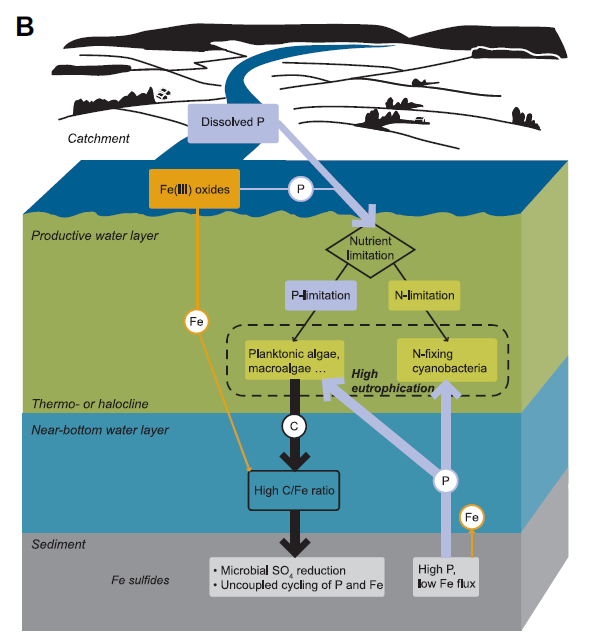
\includegraphics[scale=0.31]{../Kuvat/eutrophication_B.png}     
    \end{figure}
  \end{frame}
  
  \section{X-ray Absorption Spectroscopy}
  \begin{frame}{Small theory section}
  
  \end{frame}
  \begin{frame}{HelXAS}
  
  \end{frame}
  \begin{frame}{Measurement preparations}
  
  \end{frame}
  \section{Some early results}
  \begin{frame}{Dry soil samples}
  
  \end{frame}
  \begin{frame}{Wet aerobic soil mixed with sea water}
  
  \end{frame}
\end{document}